\documentclass[11pt]{article}
\usepackage[utf8]{inputenc}
\usepackage[T1]{fontenc}
\usepackage{amsmath}
\usepackage{amsfonts}
\usepackage{amssymb}
\usepackage[version=4]{mhchem}
\usepackage{stmaryrd}
\usepackage{graphicx}
\usepackage[export]{adjustbox}
\graphicspath{ {./images/} }

\begin{document}
Event-Driven Multistrategy Funds

Event-driven multistrategy funds diversify across a wide variety of event-driven strategies, participating in opportunities in both corporate debt and equity securities. Merger activity and debt defaults occur in waves or cycles. Merger activity is usually higher when equity returns are strong, and default rates on debt tend to rise during times of weak equity market performance. Because these two strategies are countercyclical to each other, many managers mix a number of event-driven strategies into a single fund. This combination can increase the capacity of the fund to manage higher levels of assets, as well as smooth out the opportunity set over time and various market conditions. Special situation funds invest across a number of event styles and are typically focused on equity securities, especially those with a spin-off or recent emergence from bankruptcy.

\section*{Key Observations Regarding Historical Returns of Event-Driven Multistrategy Funds}
Monthly returns to event-driven multistrategy funds are observed from January of 2000 to December of 2021 for a total of 264 observations. Statistical Summary of Returns provides univariate return statistics and partial autocorrelations of returns in the top panel, and histograms of returns in the bottom panels.

\begin{center}
\begin{tabular}{lcc}
\hline
\begin{tabular}{c}
Index (Jan. 2000- \\
Dec. 2021) \\
\end{tabular} & \begin{tabular}{c}
Credit Suisse Event- \\
Driven: \\
\end{tabular} & \begin{tabular}{c}
MSCI World \\
Equity \\
\end{tabular} \\
\hline
Annualized Arithmetic Mean & $6.5 \%$ & $6.8 \%$ \\
Annualized Standard Deviation & $7.2 \%$ & $15.4 \%$ \\
Annualized Semivolatility & $7.0 \%$ & $11.8 \%$ \\
Annualized Median & $9.2 \%$ & $15.1 \%$ \\
Skewness & -2.1 & -0.6 \\
Excess Kurtosis & 13.6 & 1.6 \\
Sharpe Ratio & 0.5 & 0.3 \\
Sortino Ratio & 0.6 & 0.4 \\
Annualized Geometric mean & $6.3 \%$ & $5.6 \%$ \\
First-Order Autocorrelation & 0.2 & 0.1 \\
Annualized Standard Deviation & $9.0 \%$ & $17.0 \%$ \\
(Adjusted for Autocorrelation) & $6.9 \%$ & $12.8 \%$ \\
Maximum & $-15.6 \%$ & $-19.0 \%$ \\
Minimum & $-18.8 \%$ & $-54.0 \%$ \\
Max Drawdown &  &  \\
\end{tabular}
\end{center}

\begin{center}
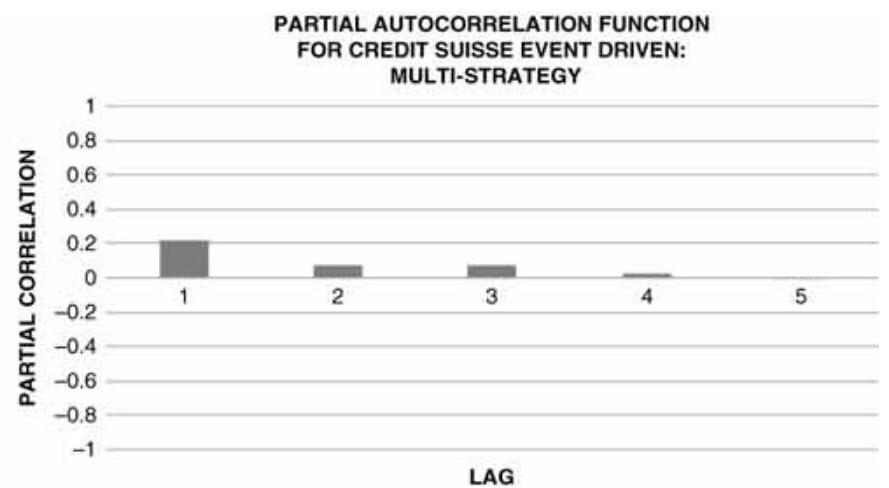
\includegraphics[max width=\textwidth]{2024_04_09_3a5f3656dbadc6becccfg-3(1)}
\end{center}

\begin{center}
\begin{tabular}{lcc}
\hline
\begin{tabular}{c}
Index (Jan. 2000- \\
Dec. 2021) \\
\end{tabular} & \begin{tabular}{c}
HFRI Event-Driven \\
(Total) \\
\end{tabular} & \begin{tabular}{c}
MSCI World \\
Equity \\
\end{tabular} \\
\hline
Annualized Arithmetic Mean & $6.8 \%$ & $6.8 \%$ \\
Annualized Standard Deviation & $6.8 \%$ & $15.4 \%$ \\
Annualized Semivolatility & $6.0 \%$ & $11.8 \%$ \\
Annualized Median & $9.4 \%$ & $15.1 \%$ \\
Skewness & -1.57 & -0.63 \\
Excess Kurtosis & 8.44 & 1.6 \\
Sharpe Ratio & 0.6 & 0.3 \\
Sortino Ratio & 0.7 & 0.4 \\
Annualized Geometric mean & $6.6 \%$ & $5.6 \%$ \\
First-Order Autocorrelation & 0.3 & 0.1 \\
Annualized Standard Deviation & $9.3 \%$ & $17.0 \%$ \\
(Adjusted for Autocorrelation) & $7.0 \%$ & $12.8 \%$ \\
Maximum & $-12.4 \%$ & $-19.0 \%$ \\
Minimum & $-24.8 \%$ & $-54.0 \%$ \\
Max Drawdown &  &  \\
\end{tabular}
\end{center}

\begin{center}
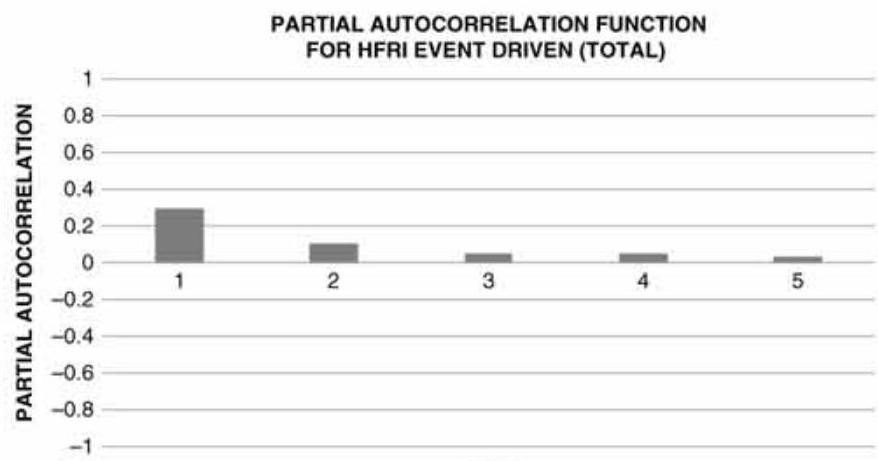
\includegraphics[max width=\textwidth]{2024_04_09_3a5f3656dbadc6becccfg-3}
\end{center}

LAG

Histogram of Credit Suisse Event Driven: Multi-Strategy Returns (Monthly) Jan. 2000-Dec. 2021

\begin{center}
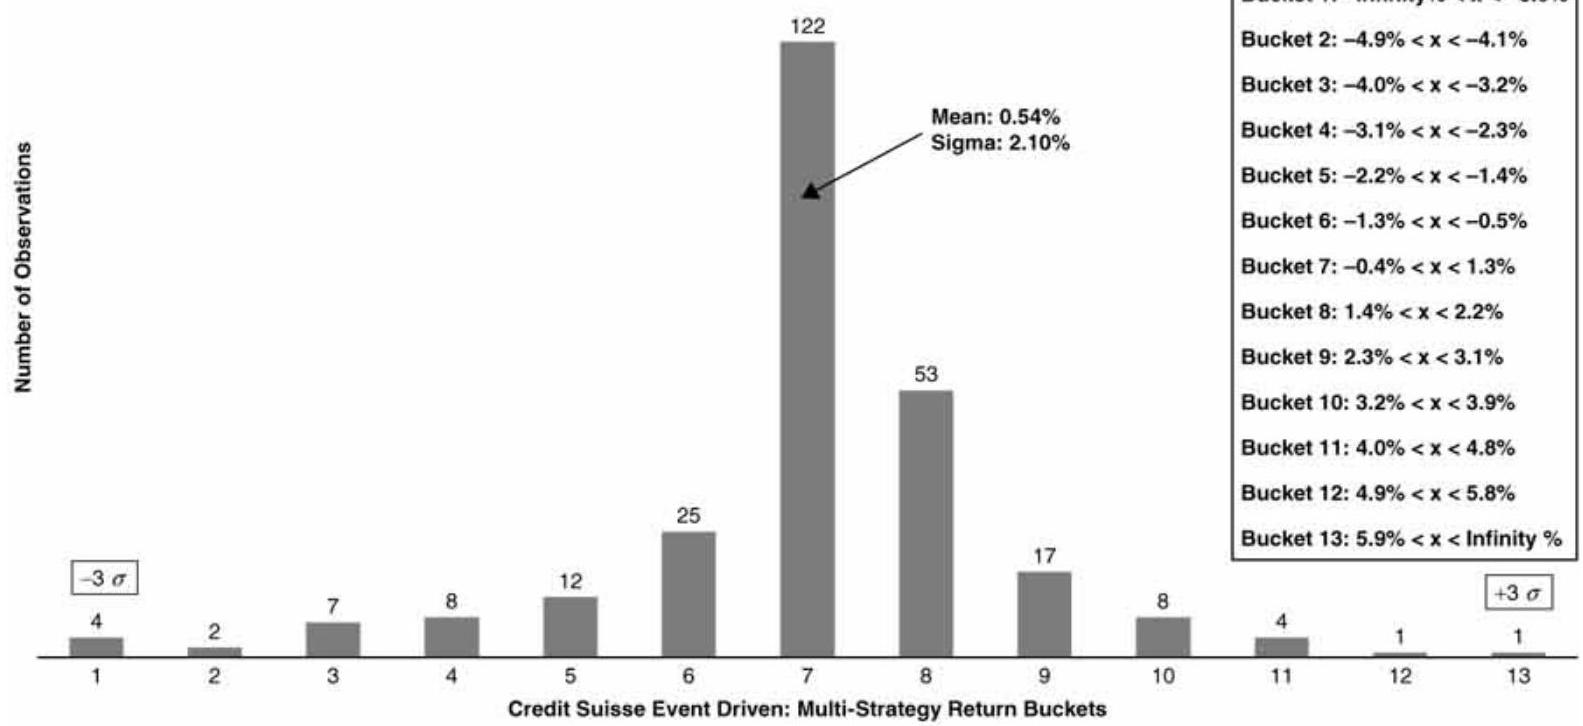
\includegraphics[max width=\textwidth]{2024_04_09_3a5f3656dbadc6becccfg-3(2)}
\end{center}

Histogram of HFRI Event Driven (Total) Returns (Monthly) Jan. 2000-Dec. 2021

\begin{center}
\begin{tabular}{l}
Bucket 1: -Infinity $\%<x<-4.9 \%$ \\
Bucket 2: $-4.8 \%<x<-4.0 \%$ \\
Bucket 3: $-3.9 \%<x<-3.1 \%$ \\
Bucket 4: $-3.0 \%<x<-2.2 \%$ \\
Bucket 5: $-2.1 \%<x<-1.3 \%$ \\
Bucket 6: $-1.2 \%<x<-0.5 \%$ \\
Bucket 7: $-0.4 \%<x<1.3 \%$ \\
Bucket 8: $1.4 \%<x<2.2 \%$ \\
Bucket 9: $2.3 \%<x<3.1 \%$ \\
Bucket 10: 3.2\%<x<3.9\% \\
Bucket 11: $4.0 \%<x<4.8 \%$ \\
Bucket 12: $4.9 \%<x<5.7 \%$ \\
Bucket 13: $5.8 \%<x<$ Infinity $\%$ \\
\hline
\end{tabular}
\end{center}

\section*{Statistical Summary of Returns}
Key observations on the returns to event-driven multistrategy funds that are consistent with economic reasoning are an essential component of knowledge and include the following:

\begin{enumerate}
  \item Event-driven multistrategy returns exhibited substantially lower volatility than world equities.

  \item Event-driven multistrategy returns exhibited somewhat fat tails and, like world equities, a negative skew.

  \item Event-driven multistrategy returns exhibited a moderate maximum drawdown, much less than world equities.

  \item Event-driven multistrategy returns exhibited some positive first-, second-, and third-order autocorrelation.

\end{enumerate}

\end{document}